This section describes the workflow used for this project, which was divided into three main steps: model prototyping, accelerator functional simulation and accelerator hardware implementation.
The tools used in each step are described in the following subsections. The goal is to expose progressively more layers of abstraction to make hardware/software co-design and debugging easier. As
can be seen in Figure \ref{fig:workflow_plan}, these three steps allow iterations to converge on a design that meets the requirements described in Section \ref{sec:prob_statement}.
\begin{figure}[H]
    \centering
    \caption{Three step workflow for designing an AI accelerator}
    \includegraphics[width=0.9\textwidth]{assets/workflow.png}
    \label{fig:workflow_plan}
\end{figure}

\subsection{Model Prototyping, Data Processing and Accuracy Measurements}
The first step in designing an accelerator is prototyping the model that the accelerator will run. Here, we prioritize productivity of development and profiling over performance. In this project,
the model was developed in TensorFlow, a widely-used Python framework maintained by Google. Its popularity implies that it has a large community of developers and is well-documented. TensorFlow
also provides a high-level API that allows for rapid prototyping of models. Furthermore, it easily converts to TensorFlow Lite, which is compatible with the Google Edge \ac{tpu} device that will
be used as a reference point of available commercial hardware. The model was developed in Python 3.11 and TensorFlow 2.14. The model was trained on the \ac{mass} SS3 dataset, which contains 62
nights of \ac{psg} recordings with 21 \ac{eeg} channels \cite*{SP3/9MYUCS_2022}. The 16-bit raw \ac{psg} data was preprocessed manually with the following steps:
\begin{itemize}
    \item Pruning of epochs of unknown sleep stage.
    \item Downsampling from 256Hz to 128Hz to reduce model size and inference energy.
    \item Filtering with 60Hz notch filter to remove noise from AC mains coupling.
    \item Filtering with 0.3-100Hz bandpass filter to remove noise (as recommended in \cite{supratak2017deepsleepnet}).
    \item Offset by half of the scale to replicate the unsigned 16-bit format expected from the \ac{adc} in the final hardware.
\end{itemize}
In addition, the two light sleep stages (N1 and N2) were merged into one stage to simplify the model. Finally, the nights were concatenated and shuffled.
All training and hyperparameter search took place on Compute Canada's Cedar cluster through remote SSH access.

Accuracy against \ac{psg} ground truth was assessed through repeated 31-fold validation: the model is trained on 60 nights and tested on the remaining two nights. The best accuracy of 5 runs is
recorded, and the process is repeated another 30 times until all pairs of nights have been tested. The training set represents 90\% of the 60 training nights. The final accuracy is the average
of the best accuracies of each validation fold. This provides measurements that are robust against night-to-night variability in the dataset. Table \ref{tab:training_hyperparameters} shows the
hyperparameters used for training the model. These have been empirically determined to yield the best accuracy with reasonable training time. Figure \ref{fig:acc_vs_epoch} shows the accuracy of
the model as a function of the number of epochs, which is shown to converge at around 100 epochs. Furthermore, Figure \ref{fig:dropout_rate} indicates that a dropout rate of 30\% is optimal for
this model.

\begin{table}[ht]
    \centering
    \renewcommand{\arraystretch}{1.2} % Vertical spacing
    \setlength{\arrayrulewidth}{1.5pt} % Thickness of vertical lines
    \caption{Training hyperparameters for vision transformer model}
    \begin{tabular}{@{} *5l @{}}
        Hyperparameter                  & Value &&&     \\\toprule
        Learning rate schedule          & $\sqrt{d_{model}}*min(\sqrt{step}, step/4000^{1.5})$ \\
        Initial learning rate           & 0.001        \\
        Batch size                      & 16            \\
        \# of epochs                    & 100           \\
        Dropout rate                    & 30\%          \\
        Class weights                   & 1.0 $\forall$ \{Wake, REM, N1/N2, N3/N4\} \\
        Optimizer                       & Adam          \\
        Data downsampling               & 256Hz → 128Hz \\
        Data filtering                  & 60Hz notch → 0.3-100Hz bandpass → 16b quantization \\            
        \hline
    \end{tabular}
    \label{tab:training_hyperparameters}
\end{table}

\begin{figure}
    \centering
    \caption{Testing set accuracy for 5 randomly-selected folds as a function of epoch}
    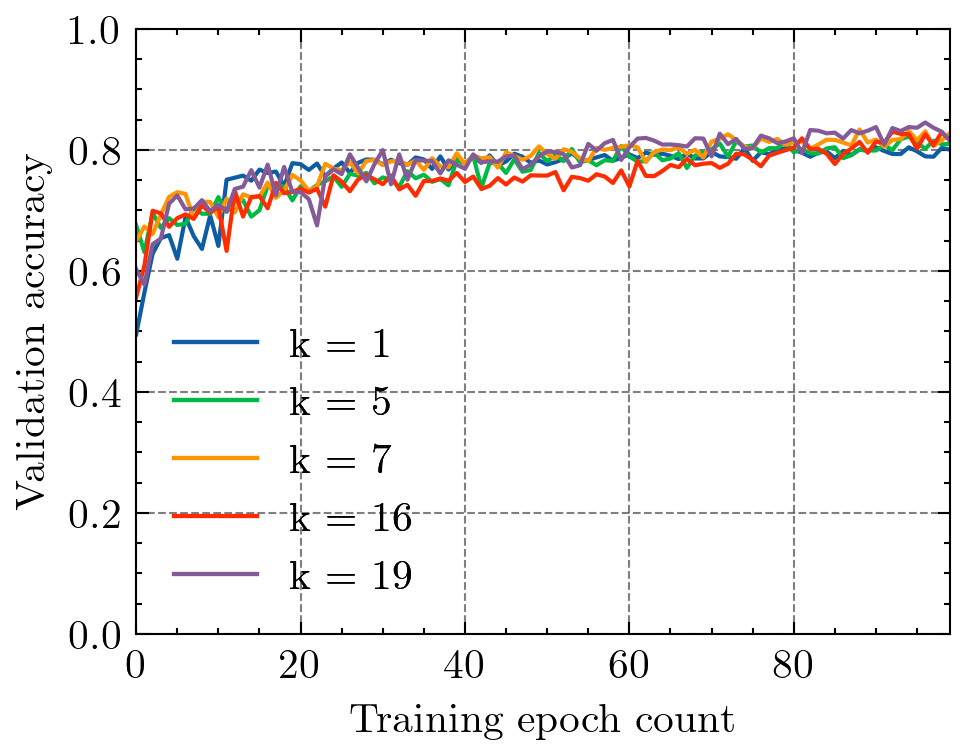
\includegraphics[width=0.9\textwidth]{assets/acc_vs_epoch/acc_vs_epoch.png}
    \label{fig:acc_vs_epoch}
\end{figure}
\begin{figure}
    \centering
    \caption{Testing set accuracy as a function of dropout rate during training}
    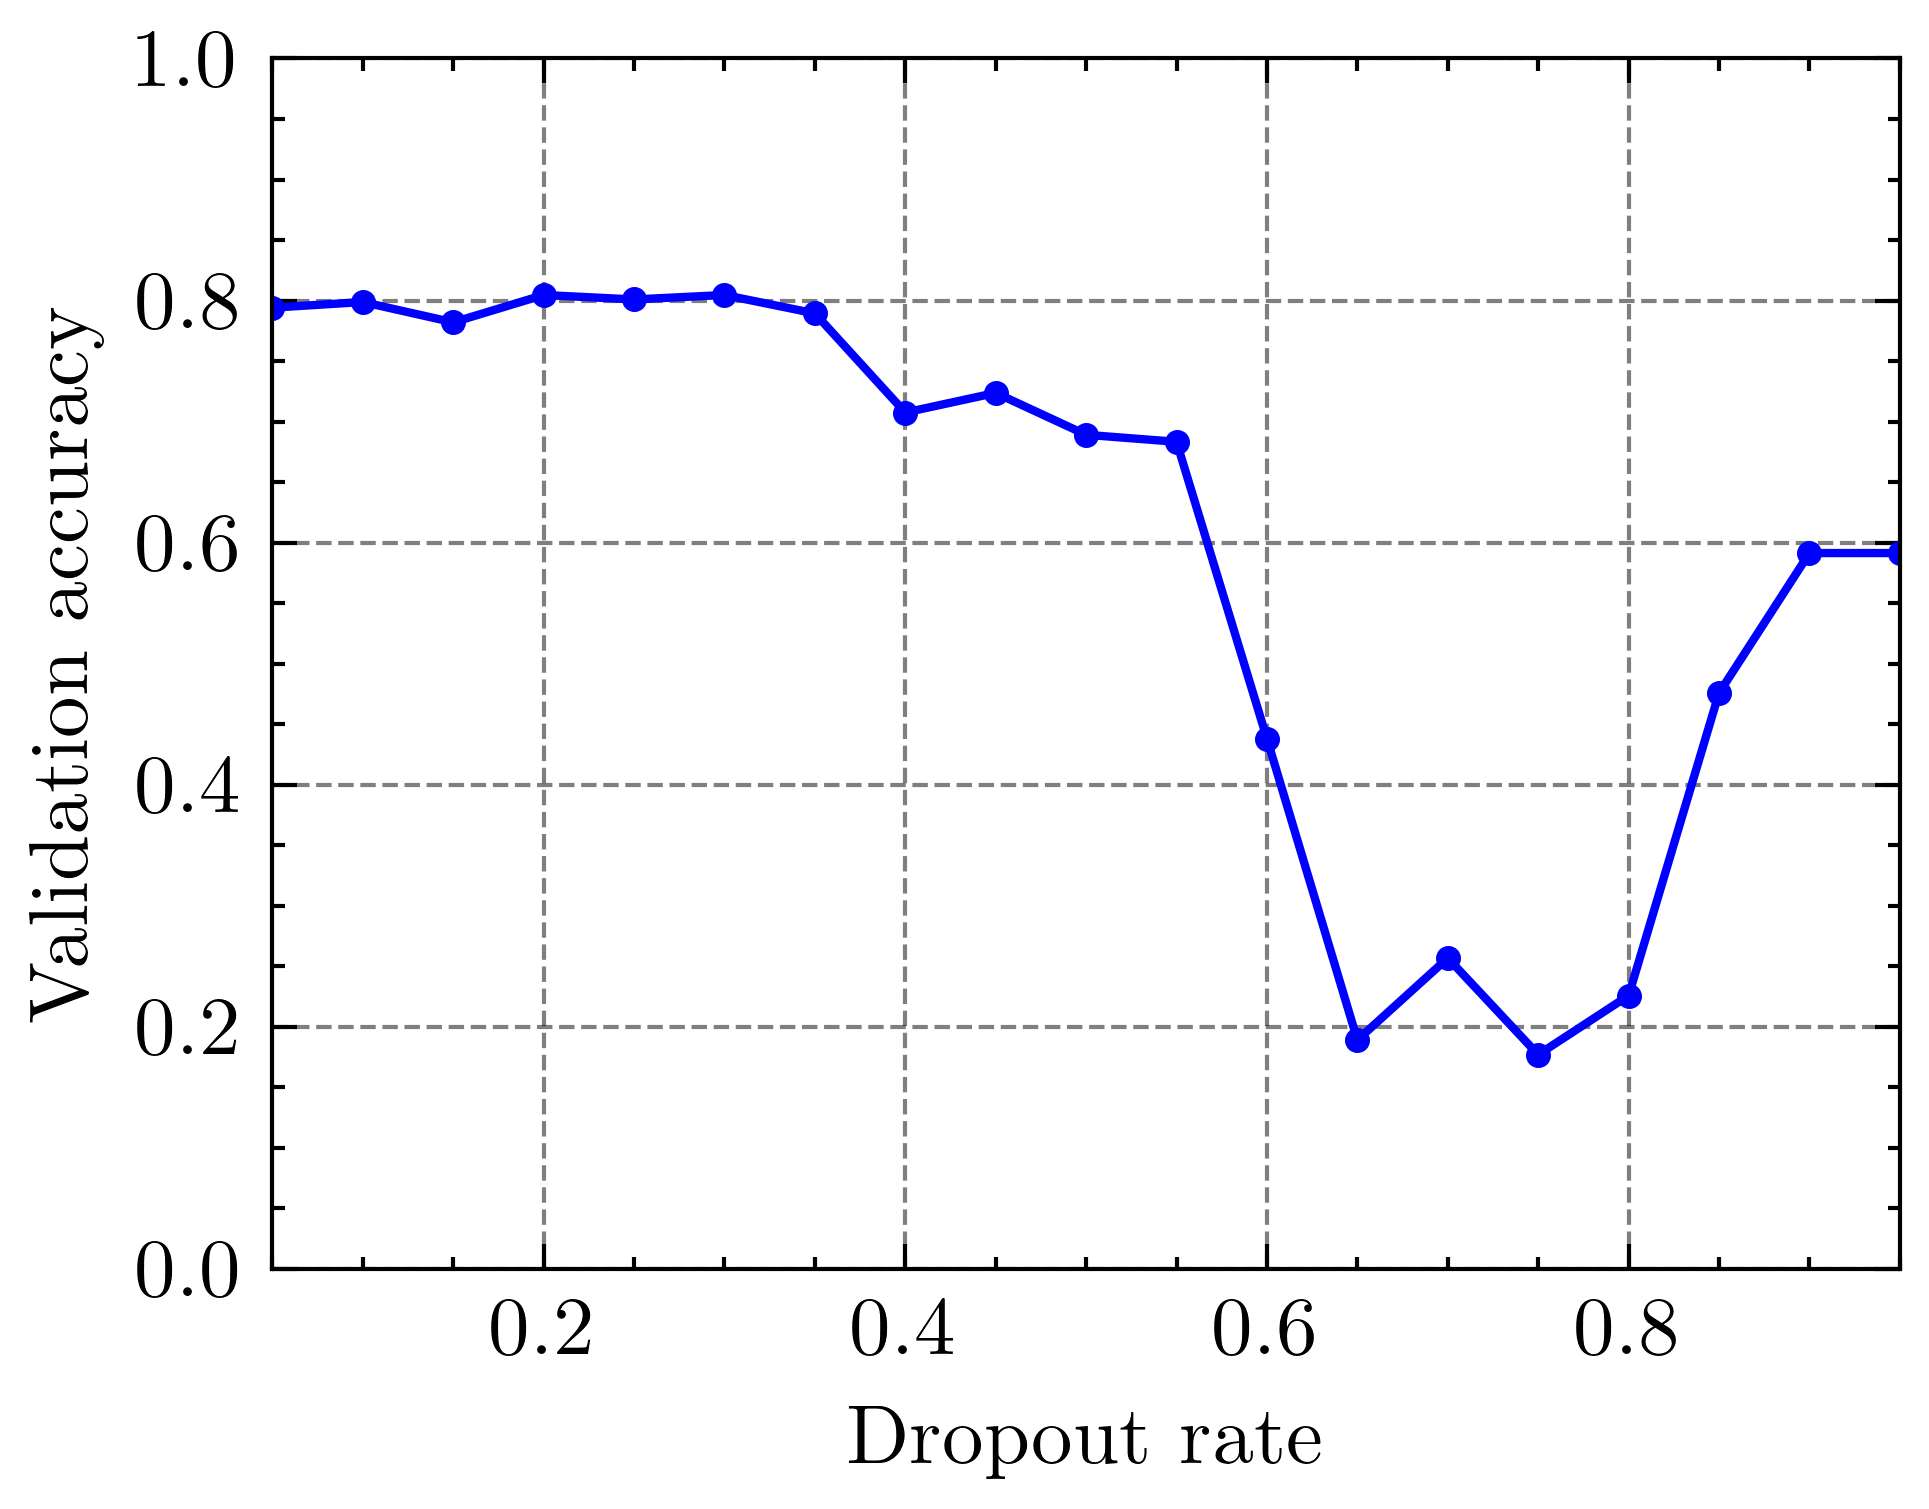
\includegraphics[width=0.9\textwidth]{assets/acc_vs_dropout_rate/acc_vs_dropout_rate.png}
    \label{fig:dropout_rate}
\end{figure}
\subsection{Accelerator Functional Simulation}
To prototype the accelerator architecture, run more accurate studies to determine the impact of design choices and write the model in a way that can be easily translated to 
hardware, a functional simulation was written. The simulation is written in C++ and, with the aim of helping subsequent SystemVerilog development, uses a similar structure to
hardware coding (cycle-level parallelism, use of FSM, limited function calls). It is organized identically to the hardware design, with a Master module that controls high-level
operation of \ac{cim} modules. It also makes use of compute modules written using the same fixed-point format and approximation as the hardware. The functional  simulation is
used to collect metrics that are more difficult to measure in high-level software or hardware, such as the distribution of inputs to certain operations, the distribution of
intermediate results, the exact number of all types of operations, etc. This information can be used to optimize the hardware design. Finally, it provides an easy way to validate
the operations by cross-checking each step with reference outputs from the TensorFlow model. The only non-standard libraries used are \texttt{armadillo} for compute verification,
\texttt{HighFive} for \ac{hdf5} file I/O (storing model parameters and \ac{eeg} data), \texttt{rapidcsv} for \ac{csv} file I/O (storing fixed-point accuracy study results and
layer output from the TensorFlow model) and \texttt{fpm} for fixed-point math.

\subsection{Accelerator Hardware Implementation}
The final step in the workflow is the hardware implementation of the accelerator. The hardware is written in SystemVerilog and uses the same structure as the functional simulation.
SystemVerilog was chosen as it provides many more ``quality of life'' features than plain Verilog, such as interfaces, typedefs, packages, assertions, etc., resulting in higher-quality
and more productive code. Several tools are used to design the hardware:
\begin{itemize}
    \item Verilator: \ac{rtl} compiler and linter.
    \item CocoTB: Python testbenching framework.
    \item GTKWave: \ac{vcd} waveform viewer.
    \item ARM Artisan Physical IP: SRAM compiler.
    \item Synopsys Design Compiler: Synthesis and performance evaluation tool.
\end{itemize}

The first three tools are open-source and compatible with all major operating systems, providing a familiar, local and OS-agnostic development environment. Testbenches are written
individually for each of the compute modules discused in Section \ref{sec:arch_compute} where multiple constrained-random inputs are passed to the modules and their output is
compared, within tolerance, to a reference values computed in software. The Master and \ac{cim} modules are tested individually with a testbench that emulates the signals and timing
that each expect from the other.

The last two tools are proprietary and are used to evaluate the performance of the design against requirements.
